\documentclass{article}
\usepackage{amsmath}
\usepackage{array}
\usepackage{color}
\usepackage{graphicx}
\usepackage{float} % utiliser H pour forcer a mettre l'image ou on veut
\usepackage{lscape} % utilisation du mode paysage
\usepackage{mathbbol} % permet d'avoir le vrai symbol pour les reels grace a mathbb
\usepackage{enumerate} % permet d'utiliser enumerate
\usepackage{moreverb} % permet d'utiliser verbatimtab : conservation la tabulation
\usepackage{stmaryrd} % permet d'utiliser \llbrackedt et \rrbracket : double crochet
\usepackage[noabbrev]{cleveref} % permet d'utiliser cref and Cref
\usepackage{caption} % permet d'utiliser subcaption
\usepackage{subcaption} % permet d'utiliser subfigure, subtable, etc


\setlength {\textwidth}{16.6cm}
\setlength {\textheight}{21cm}
\setlength {\oddsidemargin}{0cm}
\setlength{\headsep}{5pt} 

\newcommand\bn{\boldsymbol{\nabla}}
\newcommand\bo{\boldsymbol{\Omega}}
\newcommand\br{\mathbf{r}}
\newcommand\la{\left\langle}
\newcommand\ra{\right\rangle}
\newcommand\bs{\boldsymbol}
\newcommand\red{\textcolor{red}}
\newcommand\ldb{\{\!\!\{}
\newcommand\rdb{\}\!\!\}}
\newcommand\llb{\llbracket}
\newcommand\rrb{\rrbracket}

\renewcommand{\(}{\left(}
\renewcommand{\)}{\right)}
\renewcommand{\[}{\left[}
\renewcommand{\]}{\right]}


\begin{document}
\title{Diffusion}
\author{} 
\date{}
\maketitle

%%%%%%%%%%%%%%%%%%%%%%%%%%%%%%%%%%%%%%%%%%%%%%%%%%%%%%%%%%%%%%%%%%%%%%%%%%%%%%%%%%%%%%%%
\section{Introduction} \label{sec_intro}
%%%%%%%%%%%%%%%%%%%%%%%%%%%%%%%%%%%%%%%%%%%%%%%%%%%%%%%%%%%%%%%%%%%%%%%%%%%%%%%%%%%%%%%%

This paper deals with a discontinuous finite elemt spatial discretizations of the radiation 
diffusion equation on arbitrary polygonal grids, with and without adaptive mesh refinement. 
Radiation diffusion is an asymptotic limit of the radiation transport equation and can be 
written in the following form:
\begin{equation} \label{eq:radiation_diffusion}
- \div  D(\vr) \grad E(\vr) + \sigma_a(\vr) E(\vr) = Q(\vr) ,
\end{equation}
where $E$ is the radiation energy intensity, $D$ is a diffusion coefficient, $\sigma_a$ is 
an opacity coefficient, and $Q$ is the source.

Several spatial discretizations have been proposed to solve \eqt{eq:radiation_diffusion} on
arbitrary polygons (2D) and polyhedra (3D) \cite{Wachspress,PalmerLLNL,Palmer2005,MorelHall,MorelShashkov,%
BaileyAdams2008,KutnetsovMimetic}. 

Wachspress \cite{Wachspress} developed a family of rational polynomial functions that can be employed
as basis functions in a finite element method on polygonal/polyhedral grids. This yields
symmetric positive-definite (SPD) matrices but (i) the finite element integrals must be carried out 
numerically and (ii) the Jacobian of the transformation becomes zero on degenerate cells 
(such as the ones shown on \fig{fig:amr_schematics}). Palmer \cite{PalmerLLNL,Palmer2005}
proposed a node-based finite volume method that enforces particle balance over dual cells,
where a dual cell is defined as the union of all corners surrounding a given vertex $p$ and where  
a corner is a quadrilateral defined by vertex $p$, the cell center, and the midpoint
of the edges that contain vertex $p$. On a triangular grid, Palmer's scheme is equivalent 
to linear continuous finite elements with ``mass-matrix lumping''. The method is 
second-order accurate but the discretization of the diffusion equation using Palmer's method 
does not result in SPD matrices.







In this paper, we are interested in solving the diffusion equation on a
polygonal mesh. First, we want to point the usefulness of using polygonal
cells to discretize the domain of a problem. Such cell type presents a big 
advantage over traditional cells type (triangles and rectangles): polygonal 
cells allow for meshing flexibility. Boundary layer meshes can easily be set 
up, polygonal meshes can be generated from triangular meshes, and polygons 
can be included locally in existing meshes to improve mesh quality. Existing 
meshing tools such as MSTK \cite{mstk} and the Computational Geometry Algorithms 
Library \cite{cgal} may be employed to process polygonal meshes. For 
instance, the radiation transport code PDT and the CFD codes Fluent and OpenFoam 
offer polygonal mesh and solver capabilities. The following features of polygonal
cells are noteworthy:
\begin{description}
  \item[Optimal partition of the space minimizing boundary/interior ratio]
  \item[Reduced number of unknowns:] To illustrate this, we assume
    one unknown per vertex in every cell, which is standard for linear discontinuous
    finite element transport discretizations that perform well in the thick
    diffusive regime. In the 2D hexagonal example of \Cref{fig_hex_vs_tri},
    the number of unknowns would be six (one unknown per vertex). Using
    triangular cells, the same hexagon would have to be split into four
    triangles at least (thus 12 unknowns) or possibly six triangles to
    preserve symmetry (thus 18 unknowns in that case). Similarly, using
    quadrilateral cells, the hexagon would be bisected into two quadrilaterals
    at least (8 unknowns), but divisions into three of four quadrilaterals are
    also possible (thus, 12 or 16 unknowns).
    \begin{figure}[H]
      \centering
      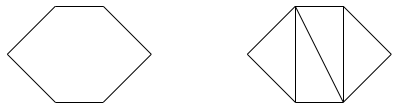
\includegraphics[width=5cm]{hex_tri_cells}
      \caption{Hexagonal cell versus triangle cells}
      \label{fig_hex_vs_tri}
    \end{figure}
  \item[Transition elements and Adaptive Mesh Refinement:] Solvers based on
    arbitrary polyhedral cells can easily handle cells with various number of
    edges. This can be particularly useful for simulations
    with Adaptive Mesh Refinement (AMR) \cite{Jessee1998,Baker2002,Wang2010a}, 
    without having to deal with the implementation of data structures to handle 
    hanging nodes \cite{Solin2008,Bangerth2007,Arnold2000}. On \Cref{fig_amr_cells}, 
    the left cell is a pentagon whereas the two cells on the right are 
    quadrilaterals. A method based on a piecewise linear discretization can
    handle locally adapted meshes without any special treatment or further
    approximation of the coupling between cells.
    \begin{figure}[H]
      \centering
      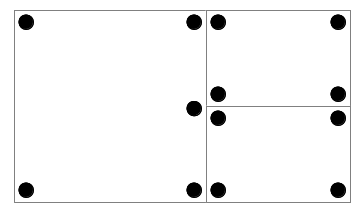
\includegraphics[width=5cm]{amr}
      \caption{AMR mesh}
      \label{fig_amr_cells}
    \end{figure}
\end{description}
Several discretization methods have been developed for arbitrary polygonal
meshes: Palmer's method \cite{Palmer2001}, mimetic finite differences
\cite{Lipnikov2004,Hyman2002,Kuznetsov2004,Brezzi2005},
Wachspress' rationale finite element \cite{Wachspress1975},
CFEM-based DFEM \cite{Warsa2008}, PWLC \cite{Bailey2008a}, PWLD 
\cite{Stone2003,Bailey2008,Bailey2008a}, and PWBLD \cite{Bailey2011}. In this
research, we focus on using PWLD to discretize the diffusion equation. The
PWLD discretization employs discontinuous finite elements and has been used to
discretize the transport equation. Using it to discretize the diffusion
equation is an important step in order to create a Diffusion Synthetic
Acceleration scheme \cite{Adams2002,Wang2010}.
In \Cref{sec_review}, we review different discretizations that can be used on
polygonal cells to discretize the diffusion equation. In \Cref{sec_ip}, we
use the PWLD finite elements to discretize the diffusion
equation. In \Cref{sec_amr}, we introduce the Adaptive Mesh Refinement
technique (AMR). In \Cref{sec_results}, we show some numerical results. We finish
in \Cref{sec_conc} by giving our conclusions.

%\section{Results} \label{sec_results}
In this Section, we compare the solution of the problem on an uniform mesh
with the one on Z-mesh \cite{Stone2003}. We also show that the
discretization used can easily handle unstructured polygonal grid. Finally, we
conclude this section with an example of AMR mesh.
\subsection{Z-mesh}
The Z-mesh is defined as in \Cref{fig_z_mesh} where $\alpha$ is a parameter
$\in [0,0.5]$. 
\begin{figure}[H]
  \centering
  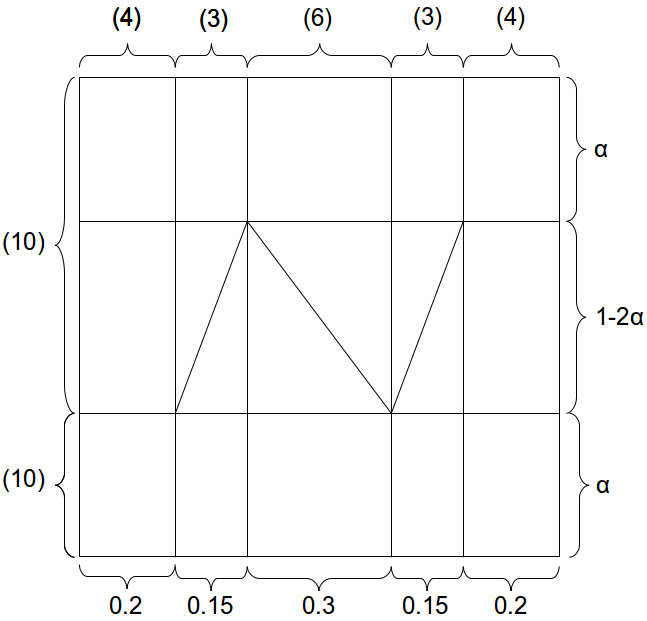
\includegraphics[width=5cm]{z_mesh}
  \caption{Z-mesh ((x) is the number of divisions and Y is the distance in cm)}
  \label{fig_z_mesh}
\end{figure}    
We compare the solution of the diffusion equation using the Z-mesh
\Cref{z_mesh_sol} with $\alpha=0.2$ with the one obtained using an uniform \Cref{u_mesh_sol}. 
The domain is 1cm by 1cm and is discretized using 20 by 20 cells. All the 
boundary conditions are vacuum. The medium is homogeneous $\Sigma_a = 0.5 cm^{-1}$ 
and $D=2$. There is a uniform source of intensity 1.                  
\begin{figure}[H]
  \centering
  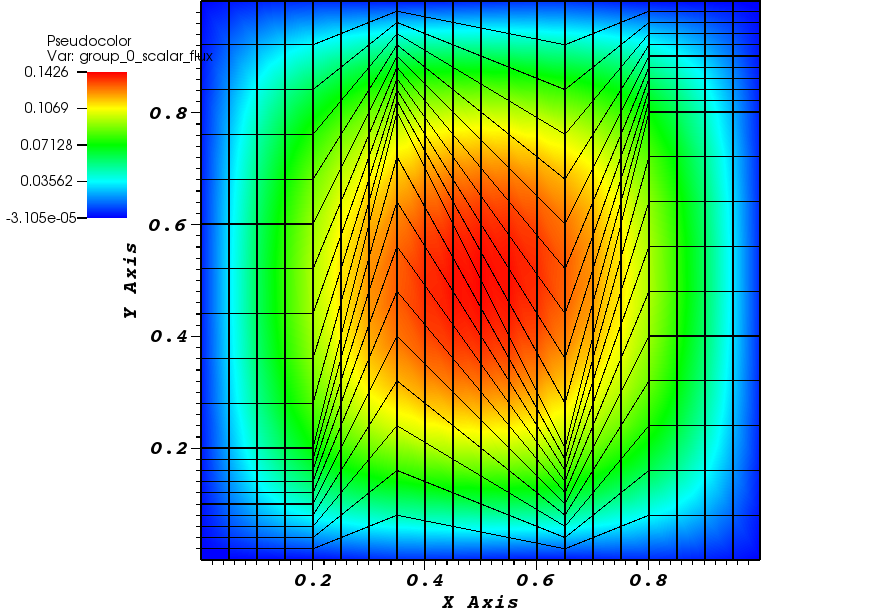
\includegraphics[width=5cm]{z_mesh_sol}
  \caption{Scalar flux on the z-mesh}
  \label{z_mesh_sol}
\end{figure}
\begin{figure}[H]
  \centering
  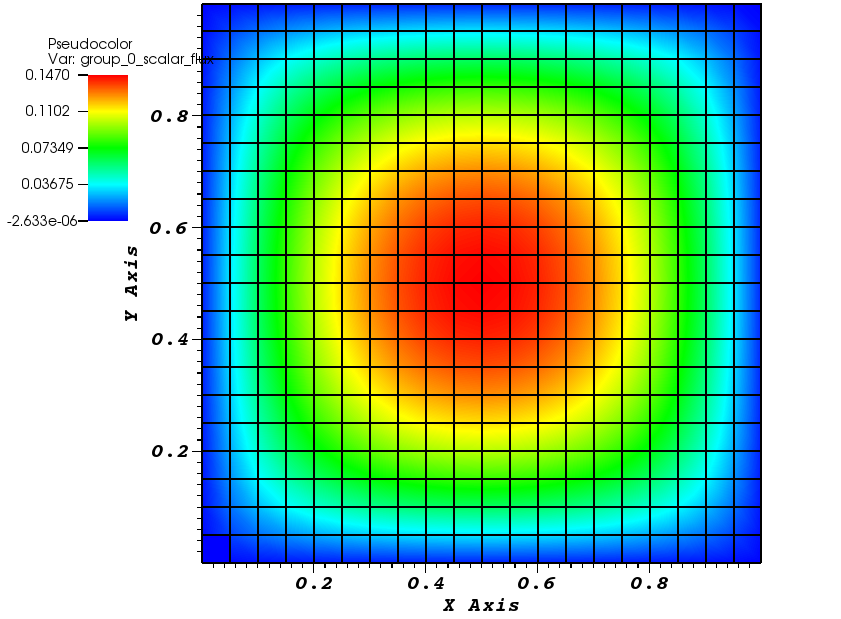
\includegraphics[width=5cm]{pwld_uniform_sol}
  \caption{Scalar flux on the uniform mesh}
  \label{u_mesh_sol}
\end{figure}
\subsection{Randomized polygonal grid}
\subsection{AMR}
The AMR problem is composed of two regions, see \Cref{amr_regions}.
\begin{figure}[H]
  \centering
  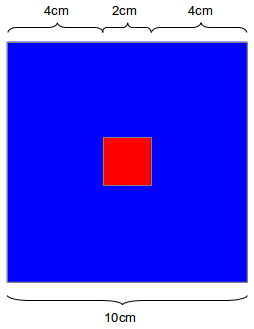
\includegraphics[width=3cm]{amr_zones}
  \caption{Regions of the AMR problem.}
  \label{amr_regions}
\end{figure}
The domain is a square of 10cm side (blue region) with in its center a smaller
square of 2cm side (red region). In the blue region, we have
$\Sigma_t=2cm^{-1}$ and $\Sigma_s=1cm^{-1}$. In the red region, we have
$\Sigma_t=1cm^{-1}$, $\Sigma_s=0.8cm^{-1}$, and a source of intensity $10
n/cm^{2}$. We use vacuum boundaries. The domain is initially discretize using
an uniform mesh of five by five cells. This mesh is then refined three
times. For each refinement, the cells with an estimated error of 70\% or more
of the largest estimated error are refined. \Cref{diffusion_amr} shows the
results.
\begin{figure}[H]
  \centering
  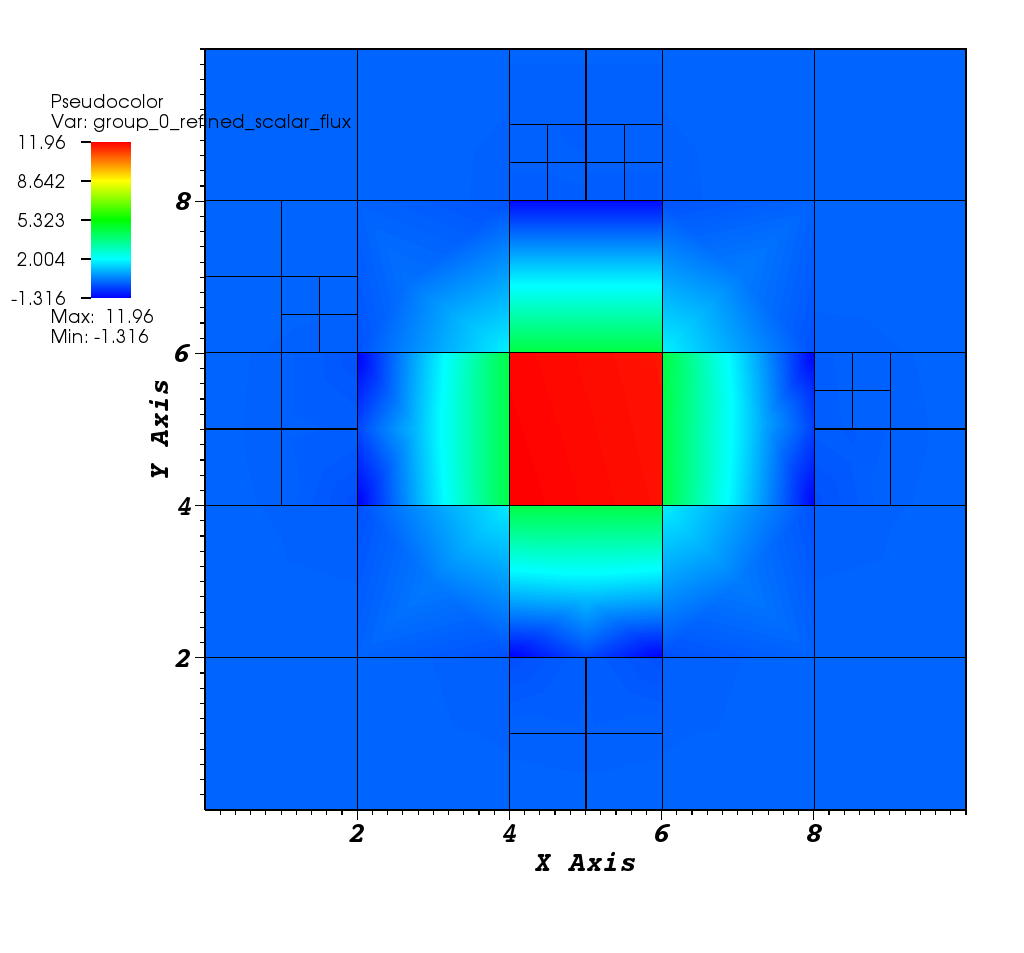
\includegraphics[width=5cm]{diffusion_amr}
  \caption{Solution of the AMR problem.}
  \label{diffusion_amr}
\end{figure}
\red{Je ne sais pas pourquoi ce ne sont pas pourquoi le raffinement est si
mauvais. Il y a surement un bug.}

%\section{Conclusions}


% bibliography
\bibliographystyle{unsrt}
\bibliography{database}


\end{document}
